\documentclass[10pt,a4paper]{article} 
\usepackage[utf8]{inputenc}
\usepackage{amsmath}
\usepackage{amsfonts}
\usepackage{amssymb}
\usepackage{graphicx}
\usepackage{epstopdf}
\usepackage[ngerman]{babel}
\usepackage[ngerman]{translator}
\usepackage{listings}
\usepackage[colorlinks=true,
        linkcolor=black,
        citecolor=black,
        filecolor=black,
        pagecolor=black,
        urlcolor=black,
        bookmarks=true,
        bookmarksopen=true,
        bookmarksopenlevel=3,
        plainpages=false,
        pdfpagelabels=true]{hyperref}


%Paket laden
\usepackage[
	nonumberlist, %keine Seitenzahlen anzeigen
	acronym,      %ein Abkürzungsverzeichnis erstellen
	toc,          %Einträge im Inhaltsverzeichnis
	section]      %im Inhaltsverzeichnis auf section-Ebene erscheinen
	{glossaries}
\usepackage{pdfpages}


\parindent 0pt
\pagestyle{headings}

%\let\oldsection\section
%\renewcommand{\section}{\newpage \oldsection}

\title{
	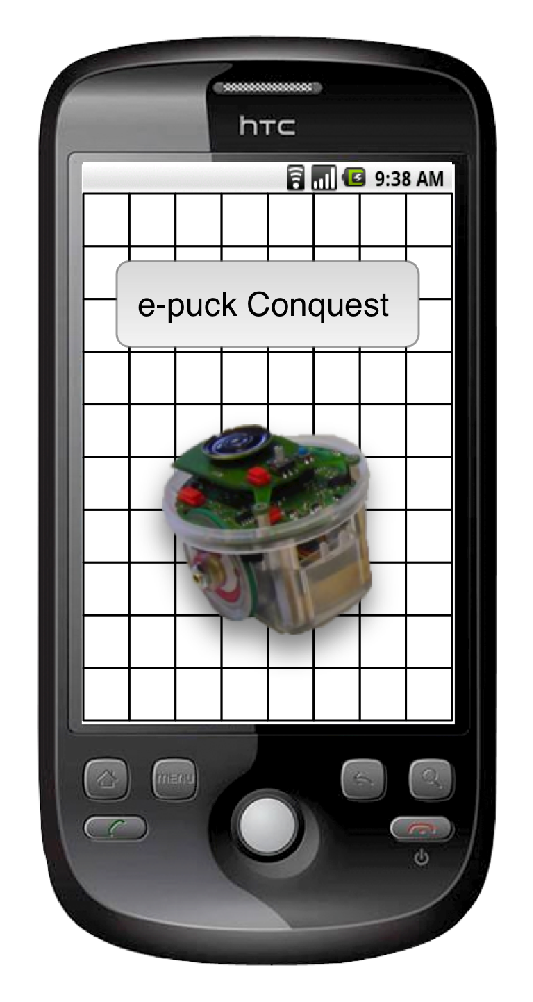
\includegraphics[height=10cm]{logo.eps} \\
%	\vspace{1cm}
	Implementierungsbericht
}
\author{
            \begin{tabular}[r]{*{3}{|c|}}
	\hline
	Phase & Verantwortlicher & E-Mail \\
	\hline \hline
	Pflichtenheft & Florian Lorenz & lorenz@fim.uni-passau.de \\
	\hline
	Entwurf & Andreas Wilhelm &  wilhelma@fim.uni-passau.de \\
	\hline
	Spezifikation & Andreas Poxrucker & poxrucke@fim.uni-passau.de \\
	\hline
	Implementierung & Martin Freund & freund@fim.uni-passau.de \\
	\hline
	Validierung & Florian Bürchner & buerchne@fim.uni-passau.de \\
	\hline
	Präsentation & Max Binder & binder@fim.uni-passau.de \\
	\hline
	\end{tabular}
}

\date{15. Dezember 2011}

	\urldef{\astern}{\url}{http://de.wikipedia.org/wiki/A*#Funktionsweise}
	
	
\begin{document}

	\maketitle
	\newpage
	\tableofcontents
	\newpage

	\begin{abstract}
		Dieses Dokument soll einen Überblick über den Ablauf der Implementierungsphase des Projekts  geben. Insbesondere sollen die Änderungen
		und Erweiterungen, die im Vergleich zum während der Entwurfs- und Spezifikationsphase vorgeschlagenen Aufbau notwendig wurden hier
		zusammengefasst und erläutert werden. Allerdings wird dabei nur auf größere bzw. strukturelle Abweichungen vom Entwurf eingegangen,
		um den Rahmen dieses Dokuments nicht zu sprengen.
	\end{abstract}	

	\section{Android Anwendung}
		\subsection{Paketaufbau}
			Während der Implementierung wurde die ursprünglich angedachte Paketstruktur erweitert, um eine bessere Übersichtlichkeit zu schaffen.
			Insbesondere wurde das Subpaket für Fahrverhalten des Logik-Threads \\(\texttt{sep.conquest.model.behaviour}) erstellt. Außerdem werden
			aufgrund des \\ \textit{Chain-Of-Responsibility}-Verhaltensmusters viele Nachrichtenklassen, sowie die entsprechenden Handlerklassen, benötigt.
			Diese wurden den beiden Subpaketen \\ \texttt{sep.conquest.model.handler} und \texttt{sep.conquest.model.requests} zugeordnet.
					
            \begin{tabular}{l|p{6cm}}
				\hline
					\textbf{Paket} & \textbf{Beschreibung} \\
				\hline \hline
					sep.conquest.activity & Aktivitätsklassen für Android Benutzeroberflächen \\
 				\hline
					sep.conquest.controller & Controller-Klasse entsprechend dem MVC-Entwurfsmuster \\
				\hline		
					sep.conquest.model & Klassen der Model-Schicht entsprechend dem MVC-Entwurfsmuster \\
				\hline	
					sep.conquest.model.behaviour & Verhaltensklassen des Logik-Threads \\
				\hline									
					sep.conquest.model.handler & Handlerklassen für Broadcast- und Bluetooth-Behandlung \\
				\hline				
					sep.conquest.model.request & Nachrichtenklassen für Broadcast- und Bluetooth-Kommunikation \\
				\hline				
					sep.conquest.util & Übergreifende Hilfsmittel \\
				\hline				
			\end{tabular}

		\subsection{Update-Mechanismus der MVC-Architektur}
			Es wurde während der Implementierung festgelegt, dass die Anwendungsdialoge (\textit{Observer}) keinen Status der e-pucks selbst halten dürfen.
			Dadurch musste die Struktur der Update-Nachrichten geändert werden. Neben der vollständigen Karte müssen auch von den Roboter-Statusinformationen
			tiefe Kopien erstellt und diese an die Dialoge gesendet werden.
			\begin{figure}[htbp]
				\centering
				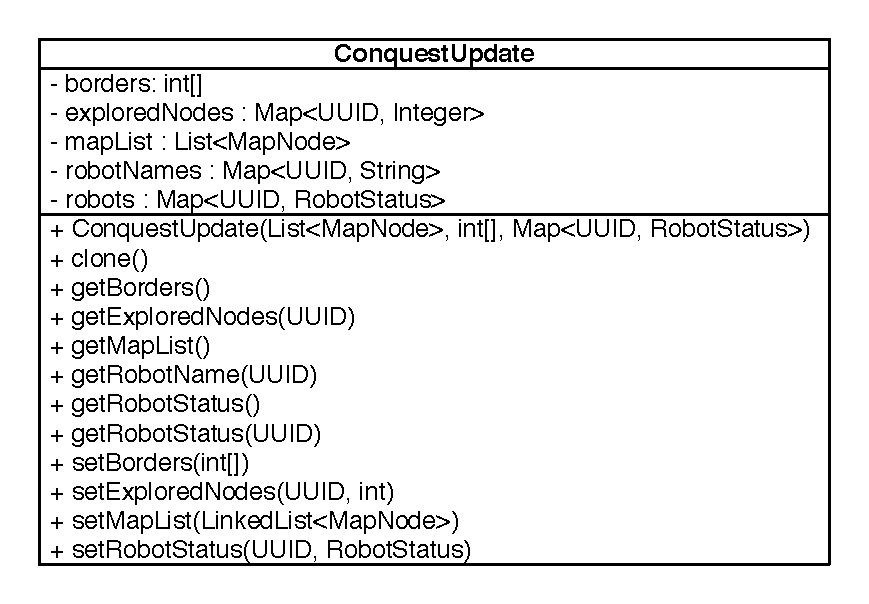
\includegraphics[width=10cm]{images/uml_ConquestUpdate.eps}
  				\caption{UML-Klassendiagramm für \texttt{ConquestUpdate}}
  				\label{fig:uml_ConquestUpdate}
  			\end{figure}				
			Um die Karte korrekt darstellen zu können, benötigt die Kartenansicht folgende Informationen:
			\begin{itemize}
				\item \textbf{\texttt{borders}} Die Grenzen des Spielfeldes, damit die Ausmaße erfasst werden können.
				\item \textbf{\texttt{exploredNodes}} Die von jedem einzelnen Roboter erkundeten Knoten. Diese Statistikdaten werden auf dem Statistik-Dialog
					angezeigt.
				\item \textbf{\texttt{mapList}} Eine Liste aller Knoten der bisher erkundeten Karte.
				\item \textbf{\texttt{robotNames}} Eine \textit{Map} aller Namen der Roboter, für die Identifizierung zur manuellen Steuerung.
				\item \textbf{\texttt{robots}} Die Statusinformationen aller Roboter inkl. Orientierung zur Darstellung.
			\end{itemize}  	
				
  		\subsection{Fabrik für Instanzen der Klassen \texttt{VirtualPuck} und \texttt{RealPuck}}
  			Durch die verschiedenartigen Roboter-Instanzen für simulierte bzw. reale Erkundung wird ein Hilfsmittel benötigt, das die jeweilige Erzeugung
  			erledigt. Die Klasse \texttt{PuckFactory} übernimmt diese Aufgabe, indem sie abhängig vom gewünschten Typ die Initialisierung durchführt.
  			Dabei müssen die \texttt{Puck}-Ableitungen am Kommunikationsmanager registriert werden, die Startpositionen und Orientierungen gesetzt sein und
  			schließlich das Handshaking initiiert werden.
  			
  		\subsection{Erweiterungen des Simulators}
			Um die Simulation der Roboter entsprechend den realen Vorbildern gestalten zu können, mussten gegenüber dem Entwurf einige Änderungen gemacht werden.
			Der Simulator hält je virtuellem Puck eine Instanz der Klasse \texttt{SimRobot}, welche die Zustände der Roboter speichert. Ein Timer steuert den
			Ablauf der Nachrichtenkommunikation, wobei sichergestellt wird, dass jeder Roboter gleichmäßig Nachrichten entgegennimmt und versendet. Damit auch
			Kollisionen vom Simulator berücksichtigt werden können, sind Fahranweisungen zum nächsten Knoten in 3 Schritten auszuwerten. Sollten sich zwei
			simulierte Roboter auf dem Weg zu einem Knoten auf der selben Position (in 1/3 Schritten) befinden, so wird eine Kollision gemeldet und zum zuletzt
			besuchten Knoten zurückgefahren.
  		
			\begin{figure}[htbp]
				\centering
				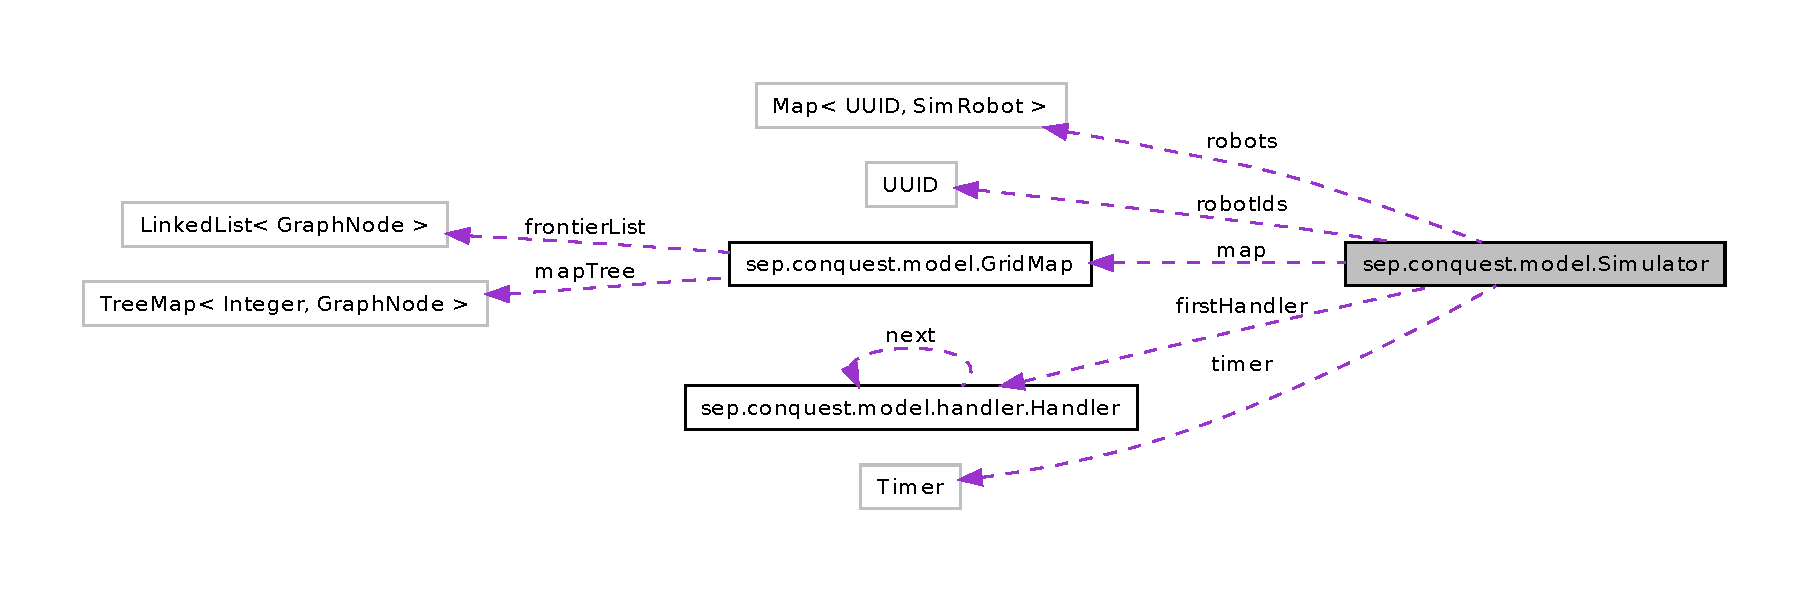
\includegraphics[width=12cm]{images/call_Simulator.pdf} 
  				\caption{Verwendungen von Klasse \texttt{Simulator}}
  				\label{fig:call_Simulator}
  			\end{figure}  		
  			
  		\subsection{Implementierte Verhaltensklassen}
  			Die Verhaltensklassen steuern das Fahrverhalten der Roboter und werden je nach deren Zustand (Initialisierung, Lokalisierung, Erkundung, Rückkehr)
  			aktiviert. Die Klasse \texttt{LogicThread} hält den ersten Eintrag einer Liste von entsprechenden Verhaltensklassen. Beim Wechsel eines Zustands
  			wird die Klasse \texttt{BehaviourFactory} verwendet, um eine neue Liste zu laden. \\
  			Es existieren folgende Verhaltensklassen:
  			
  			\textbf{Initialisierung}
			\begin{itemize}
				\item \textbf{\texttt{IdleBehaviour}} In dem Verhalten wird für 5 Sekunden auf eingehende Handshaking-Nachrichten reagiert, um sämtliche
					Teilnehmer zu berücksichtigen.
			\end{itemize}  
  			\textbf{Lokalisierung}
			\begin{itemize}
				\item \textbf{\texttt{LocalLocalizeBehaviour}} Hier werden die Startpositionen und Orientierungen der Roboter gesetzt. Außerdem wird der Knotentyp
					des realen bzw. virtuellen Roboters angefordert und bei Erhalt gespeichert.
			\end{itemize}
  			\textbf{Erkundung}
			\begin{itemize}
				\item \textbf{\texttt{RemovePathlessBehaviour}} Nicht erreichbare Frontier-Knoten werden entfernt.
				\item \textbf{\texttt{DistanceBehaviour}} Mit Hilfe des A*-Algorithmus werden Entfernungen zu den Frontier-Knoten ermittelt.
				\item \textbf{\texttt{InnerBehaviour}} Frontier-Knoten, welche vollständig von bereits erkundeten Knoten liegen, werden als weniger günstig
					eingestuft.
				\item \textbf{\texttt{CooperativeBehaviour}} Frontier-Knoten, welche bereits andere Teilnehmer erkunden, werden als weniger günstig eingestuft.
			\end{itemize} 							
  			\textbf{Rückkehr}
			\begin{itemize}
				\item \textbf{\texttt{ReturnBehaviour}} Es wird mit Hilfe des A*-Algorithmus der kürzeste Rückweg ermittelt.
			\end{itemize} 			
					
		\subsection{Implementierte Handlerklassen und Nachrichtenklassen}
			Die Nachrichtenkommunikation innerhalb der Anwendung und mit dem realen e-puck wurde vollständig durch das \textit{Chain-Of-Responsibility}
			Entwurfsmuster realisiert. Es wurden folgende Handlerklassen (mit entsprechenden Nachrichtenklassen) verwendet:
			
		 	\textbf{Broadcast-Kommunikation der \texttt{Puck}-Ableitungen}
			\begin{itemize}
				\item \textbf{\texttt{CollisionRequestHandler (CollisionRequest)}} Sobald eine Kollisionsmeldung eines anderen Teilnehmers empfangen wird,
					registriert der Puck diesen Zustand in seinen gespeicherten \texttt{RobotStatus} Instanzen.
				\item \textbf{\texttt{ControlledRequestHandler (ControlledRequest)}} Es wird am zugehörigen Puck registriert, dass eine manuelle Steuerung
					des Benutzers aktiv ist.
				\item \textbf{\texttt{DriveRequestHandler (DriveRequest)}} Eine Steueranweisung des Benutzers wird entgegengenommen und die entsprechenden
					Kommandos an den Puck weitergereicht.
				\item \textbf{\texttt{FailureRequestHandler (FailureRequest)}} Fehlermeldungen werden analysiert und die entsprechenden Zustandsvariablen
					an der Puck-Instanz gesetzt.		
				\item \textbf{\texttt{HelloRequestHandler (HelloRequest)}} Handshaking-Nachrichten werden empfangen und ggf. an alle Teilnehmer weitergegeben.	
				\item \textbf{\texttt{IntentRequestHandler (IntenRequest)}} Von einem anderen Teilnehmer wurde ein beabsichtigter Zielknoten empfangen, diese
					Information wird unter anderem bei der kooperativen Auswahl des nächsten Frontier-Knoten benötigt.
				\item \textbf{\texttt{SpeedRequestHandler (SpeedRequest)}} Eine Änderung der Fahrgeschwindigkeit wird vom Benutzer gesendet. Diese wird an
					die entsprechende Puck-Instanz weitergereicht und der Zustand an die anderen Teilnehmer gesendet.				
				\item \textbf{\texttt{StatusUpdateRequestHandler (StatusUpdateRequest)}} Es wird eine Aktualisierungsnachricht eines anderen Teilnehmers
					registriert.		
			\end{itemize}  
		 	\textbf{Bluetooth-Kommunikation der \texttt{RealPuck}-Instanzen}
			\begin{itemize}
				\item \textbf{\texttt{PuckAbyssHandler (PuckRequest)}} Es wurde ein Abgrund gemeldet. Die Position wird auf den letzten Knoten und die
					Orientierung entgegengesetzt der letzten gesetzt.
				\item \textbf{\texttt{PuckCollisionHandler (PuckRequest)}} Es wurde eine Kollision gemeldet. Die Position wird auf den letzten Knoten und die
					Orientierung entgegengesetzt der letzten gesetzt.					
				\item \textbf{\texttt{PuckNodeHitHandler (PuckRequest)}} Der e-puck meldet die Erkundung eines Knoten. Dieser wird in die lokale Karte
					eingetragen und an sämtliche Teilnehmer gesendet.
				\item \textbf{\texttt{PuckOKHandler (PuckRequest)}} Der e-puck meldet die Ausführung seiner letzten Anweisung, die keine spezielle Antwort
					benötigt. Ein Beispiel dafür ist eine Drehanweisung. Die OK-Nachricht bewirkt den nächsten Schritt des Logik-Threads.
				\item \textbf{\texttt{PuckStatusHandler (PuckRequest)}} Es wird der aktuelle Status (nach Anforderung) vom e-puck gesendet. Dieser Status wird
					lokal gespeichert und auch an die anderen Teilnehmer gesendet.
			\end{itemize} 
		 	\textbf{Interne Kommunikation von \texttt{SimRobot}-Instanzen}
			\begin{itemize}
				\item \textbf{\texttt{SimLEDHandler (VirtualPuckRequest)}} Steuerungen der LEDs werden am Simulator in einfache Bestätigungsmeldungen (OK)
					umgesetzt und zurückgesendet.
				\item \textbf{\texttt{SimResetHandler (VirtualPuckRequest)}} Reset-Anforderungen werden vom \texttt{SimRobot} umgesetzt.
				\item \textbf{\texttt{SimSpeedHandler (VirtualPuckRequest)}} Änderungen der Geschwindigkeit werden am Simulator in einfache Bestätigungsmeldungen
					(OK) umgesetzt und zurückgesendet.
				\item \textbf{\texttt{SimStatusHandler (VirtualPuckRequest)}} Liefert den geforderten Zustand (Position, Orientierung, usw.).
				\item \textbf{\texttt{SimTurnHandler (VirtualPuckRequest)}} Initiiert eine Drehung der \texttt{SimRobot}-Instanz und gibt anschließend eine
					Bestätigungsmeldung (OK) zurück.																		
			\end{itemize}  		
			
	\section{e-puck}
	
	\section{Implementierungsaufwand}
		\subsection{Android Anwendung}
		\begin{tabular}{|l|l|l|}
			\hline \textbf{Tätigkeit} & \textbf{Arbeitsaufwand} (Plan) & \textbf{Arbeitsaufwand} (Ist) \\ 
			\hline Controller & 5 Std. & 5 Std. \\ 
			\hline Environment & 10 Std. & 10 Std. \\ 
			\hline Pucks & 35 Std. & 20 Std. \\ 
			\hline GridMap & 30 Std. & 35 Std. \\ 
			\hline MapSurfaceView & 30 Std. & 40 Std. \\ 
			\hline Connect Activity & 20 Std. & 10 Std. \\ 
			\hline Bluetooth Suche & 5 Std. & 5 Std. \\ 
			\hline Benutzeroberfläche (sonst.) & 12 Std. & 15 Std. \\ 
			\hline Statistik Activity & 6 Std. & 10 Std. \\ 
			\hline Handler & 10 Std. & 20 Std. \\ 
			\hline Komm.-Manager & 5 Std. & 3 Std. \\ 
			\hline Nachrichten & 5 Std. & 3 Std. \\ 
			\hline Logik & 20 Std. & 30 Std. \\ 
			\hline Simulator & 18 Std. & 15 Std. \\ 
			\hline Simulator Activity & 12 Std. & 5 Std. \\ 
			\hline Anbindung (Simulator) & 12 Std. & 10 Std. \\ 
			\hline Abstimmung Broadcast & 15 Std. & 10 Std. \\ 
			\hline Abstimmung Clients & 15 Std. & 15 Std. \\ 
			\hline Abstimmung Handler & 18 Std. & 30 Std \\ 
			\hline Abstimmung Karte & 12 Std. & 15 Std. \\ 
			\hline Abstimmung Export & 10 Std. & 5 Std. \\ 
			\hline Abstimmung Steuerung & 20 Std. & 20 Std. \\ 
			\hline \textbf{Summe} & \textbf{325 Std.} & \textbf{331 Std.} \\ 
			\hline 
		\end{tabular} 
		
		\subsection{e-puck}
		\begin{tabular}{|l|l|l|}
			\hline \textbf{Tätigkeit} & \textbf{Arbeitsaufwand} (Plan) & \textbf{Arbeitsaufwand} (Ist) \\ 
			\hline Interrupt & 10 Std. & 15 Std. \\ 
			\hline Kommunikation & 30 Std. & 35 Std. \\ 
			\hline ADC & 10 Std. & 15 Std. \\ 
			\hline I2C-Bus & 15 Std. & 20 Std. \\ 
			\hline Sensoren Abstand & 20 Std. & 15 Std. \\ 
			\hline Sensoren Linien & 15 Std. & 20 Std. \\ 
			\hline Subsumption 1 & 25 Std. & 30 Std. \\ 
			\hline Subsumption 2 & 25 Std. & 35 Std. \\ 
			\hline Abstimmung & 5 Std. & 10 Std. \\ 
			\hline Echtzeituhr & 5 Std. & 5 Std. \\ 
			\hline \textbf{Summe} & \textbf{160 Std.} & \textbf{200 Std.} \\ 
			\hline 
		\end{tabular} 
				 			
\end{document}
